\documentclass[11pt,a4paper]{article}

% Typography and page layout
\usepackage[T1]{fontenc}
\usepackage[utf8]{inputenc}
\usepackage{lmodern}
\usepackage[margin=2.6cm]{geometry}
\usepackage{microtype}
\usepackage{amsmath,amssymb}
\usepackage{xcolor}
\usepackage{titlesec}
\usepackage{fancyhdr}
\usepackage[hidelinks]{hyperref}
\usepackage{graphicx}

\definecolor{accent}{HTML}{264653}
\setlength{\parindent}{0pt}
\setlength{\parskip}{0.6em}
\linespread{1.06}
\titleformat{\section}{\large\sffamily\bfseries\color{accent}}{\thesection}{0.7em}{}
\titlespacing*{\section}{0pt}{1.3em}{0.5em}
\pagestyle{fancy}
\fancyhf{}
\fancyfoot[L]{\small\sffamily\color{accent}Robbe Van Haverbeke}
\fancyfoot[R]{\small\sffamily\thepage}
\renewcommand{\headrulewidth}{0pt}
\renewcommand{\footrulewidth}{0.3pt}

\title{Lineair response assumption}
\author{Robbe Van Haverbeke}
\date{September 2026}
\hypersetup{pdftitle={Lineaire responsaanname},pdfauthor={Robbe Van Haverbeke}}

\begin{document}

\begin{center}
    {\LARGE\sffamily\bfseries\color{accent}Lineaire responsaanname\par}
    \vspace{0.6em}
    {\normalsize Robbe Van Haverbeke\par}
    \vspace{0.2em}
    {\small\color{gray}September 2026\par}
\end{center}
\vspace{0.3em}
{\color{accent}\hrule height 0.8pt}
\vspace{0.5em}

\section{Context}
For a bimolecular system, a probe and a target can bind to form a
probe--target complex. The kinetics are governed by
\begin{equation}
    \dot{x}=k^+(a-x)(c-x)-k^-x.
    \label{eq:kinetics}
\end{equation}
Here, $x$ is the concentration of bound complex, while $a$ and $c$ are
the initial total concentrations of probe and target, respectively.
The parameters $k^+$ and $k^-$ are the association and dissociation
rate constants.

\section{Equilibrium}
At equilibrium, $x=x_0$ and $\dot{x}=0$. Equation~\eqref{eq:kinetics}
therefore gives
\begin{equation}
    0=k^+x_0^2-\bigl[k^+(a+c)+k^-\bigr]x_0+k^+ac.
    \label{eq:equilibrium}
\end{equation}
Defining the dissociation constant as
\begin{equation}
    K_d=\frac{k^-}{k^+},
\end{equation}
the physical solution, satisfying $0\leq x_0\leq\min(a,c)$, is
\begin{equation}
    \boxed{\displaystyle
    x_0=\frac{1}{2}\left[a+c+K_d-\sqrt{(a+c+K_d)^2-4ac}\right].}
    \label{eq:x0}
\end{equation}

\section{Perturbation around equilibrium}
For a deviation from equilibrium, we write
\begin{equation}
    x=x_0+\Delta x.
\end{equation}
Keeping the rate constants fixed, substitution into
Equation~\eqref{eq:kinetics} yields
\begin{equation}
\begin{aligned}
    \frac{\mathrm{d}\Delta x}{\mathrm{d}t}
    ={}&\underbrace{k^+x_0^2-\bigl[k^+(a+c)+k^-\bigr]x_0+k^+ac}
        _{=\,0\;\text{at equilibrium}}\\[0.8em]
       &-\bigl[k^+(a+c-2x_0)+k^-\bigr]\Delta x
        +k^+(\Delta x)^2.
\end{aligned}
\end{equation}
Hence, the exact perturbation equation simplifies to
\begin{equation}
    \boxed{\displaystyle
    \frac{\mathrm{d}\Delta x}{\mathrm{d}t}
    =-\bigl[k^+(a+c-2x_0)+k^-\bigr]\Delta x
     +k^+(\Delta x)^2.}
    \label{eq:perturbation}
\end{equation}
The linear approximation follows by neglecting the quadratic term
$k^+(\Delta x)^2$ for sufficiently small deviations. The rest of this document will consist of an analysis detailing if this neglect of a quadratic response is justified. This linear assumption will lead to the possibility of using linear response theory on the periodically perturbed system, which will greatly facilitate further analysis and parameter extraction.
\section{Relaxation rates}
\subsection{Linear response}

For sufficiently small deviations from equilibrium, the quadratic term
in Equation~\eqref{eq:perturbation} can be neglected, giving
\begin{equation}
    \frac{\mathrm{d}\Delta x}{\mathrm{d}t}
    = -\bigl[k^+(a+c-2x_0)+k^-\bigr]\Delta x.
\end{equation}
The deviation therefore decays exponentially,
\begin{equation}
    \Delta x(t)=\Delta x(0)e^{-\lambda_1 t},
\end{equation}
with relaxation rate
\begin{equation}
    \boxed{\lambda_1 = k^+S,}
\end{equation}
where
\begin{equation}
    S = a+c+K_d-2x_0
      = \sqrt{(a+c+K_d)^2-4ac}.
\end{equation}

\subsection{Quadratic response}

When the quadratic term cannot be neglected,
Equation~\eqref{eq:perturbation} can be written as
\begin{equation}
    \frac{\mathrm{d}\Delta x}{\mathrm{d}t}
    = -k^+S\Delta x+k^+(\Delta x)^2
    = -k^+(S-\Delta x)\Delta x.
\end{equation}
Unlike the linear case, the deviation no longer follows a single
exponential decay. Instead, we can define an instantaneous
relaxation rate through
\begin{equation}
    \frac{\mathrm{d}\Delta x}{\mathrm{d}t}
    = -\lambda_{\mathrm{2}}(\Delta x)\Delta x,
\end{equation}
which gives
\begin{equation}
    \boxed{\lambda_{\mathrm{2}}(\Delta x)
    = k^+(S-\Delta x)
    = \lambda_1\left(1-\frac{\Delta x}{S}\right).}
\end{equation}
The relaxation rate thus depends on the deviation from equilibrium:
it is lower than $\lambda_1$ for $\Delta x>0$ and higher for
$\Delta x<0$. As the system approaches equilibrium,
$\lambda_{\mathrm{2}}\to\lambda_1$.

\section{Estimation of error}
The  magnitude of the $\frac{\Delta x}{S}$ term directly tells us how closely the complete system can be approximated with an exponential decay. As seen in equation (\ref{eq:x0}), $x_0$ can be expressed in function of experimentally accessible parameters. $\Delta x$ is not directly accessible, but I estimate it as the difference between equilibrium concentrations at $T_0$ and $T_0 + \epsilon$. This is an over-estimation, as this only happens in the case of $\omega \rightarrow 0$ (at the upper frequency of our measuring range, we would only get about 40\% of this value), but this gives a viable upper boundary of the error.

Using these conventions we can write $\Delta x$ as follows, with \(\Delta K_d=K_d(T_{\mathrm{high}})-K_d(T_{\mathrm{low}})\)

\begin{equation}
\begin{aligned}
\Delta x
&= x_0(T_{\mathrm{high}})-x_0(T_{\mathrm{low}})\\
&= \frac{1}{2}\left[
\Delta K_d
-\sqrt{\bigl(a+c+K_d(T_{\mathrm{high}})\bigr)^2-4ac}
+\sqrt{\bigl(a+c+K_d(T_{\mathrm{low}})\bigr)^2-4ac}
\right].
\end{aligned}
\end{equation}

To estimate the error we can then define

\begin{equation}
    \boxed{\frac{\Delta x}{S} = \frac{\Delta K_d
-\sqrt{\bigl(a+c+K_d(T_{\mathrm{high}})\bigr)^2-4ac}
+\sqrt{\bigl(a+c+K_d(T_{\mathrm{low}})\bigr)^2-4ac}}{2\sqrt{(a+c+K_d^0)^2-4ac}}}
\end{equation}

Then, using experimentally defined values of $a = 0.5$ µM, $T_0 = 33.5^\circ C$, $\Delta T = 1^\circ C$, $K_{d,0} = 0.6524$ µM and $\Delta K_d =0.20$ µM, we find the ratio between the two relaxation rates. This ratio is plotted against the target concentration in figure \ref{fig:ratio}.
\begin{figure}
    \centering
    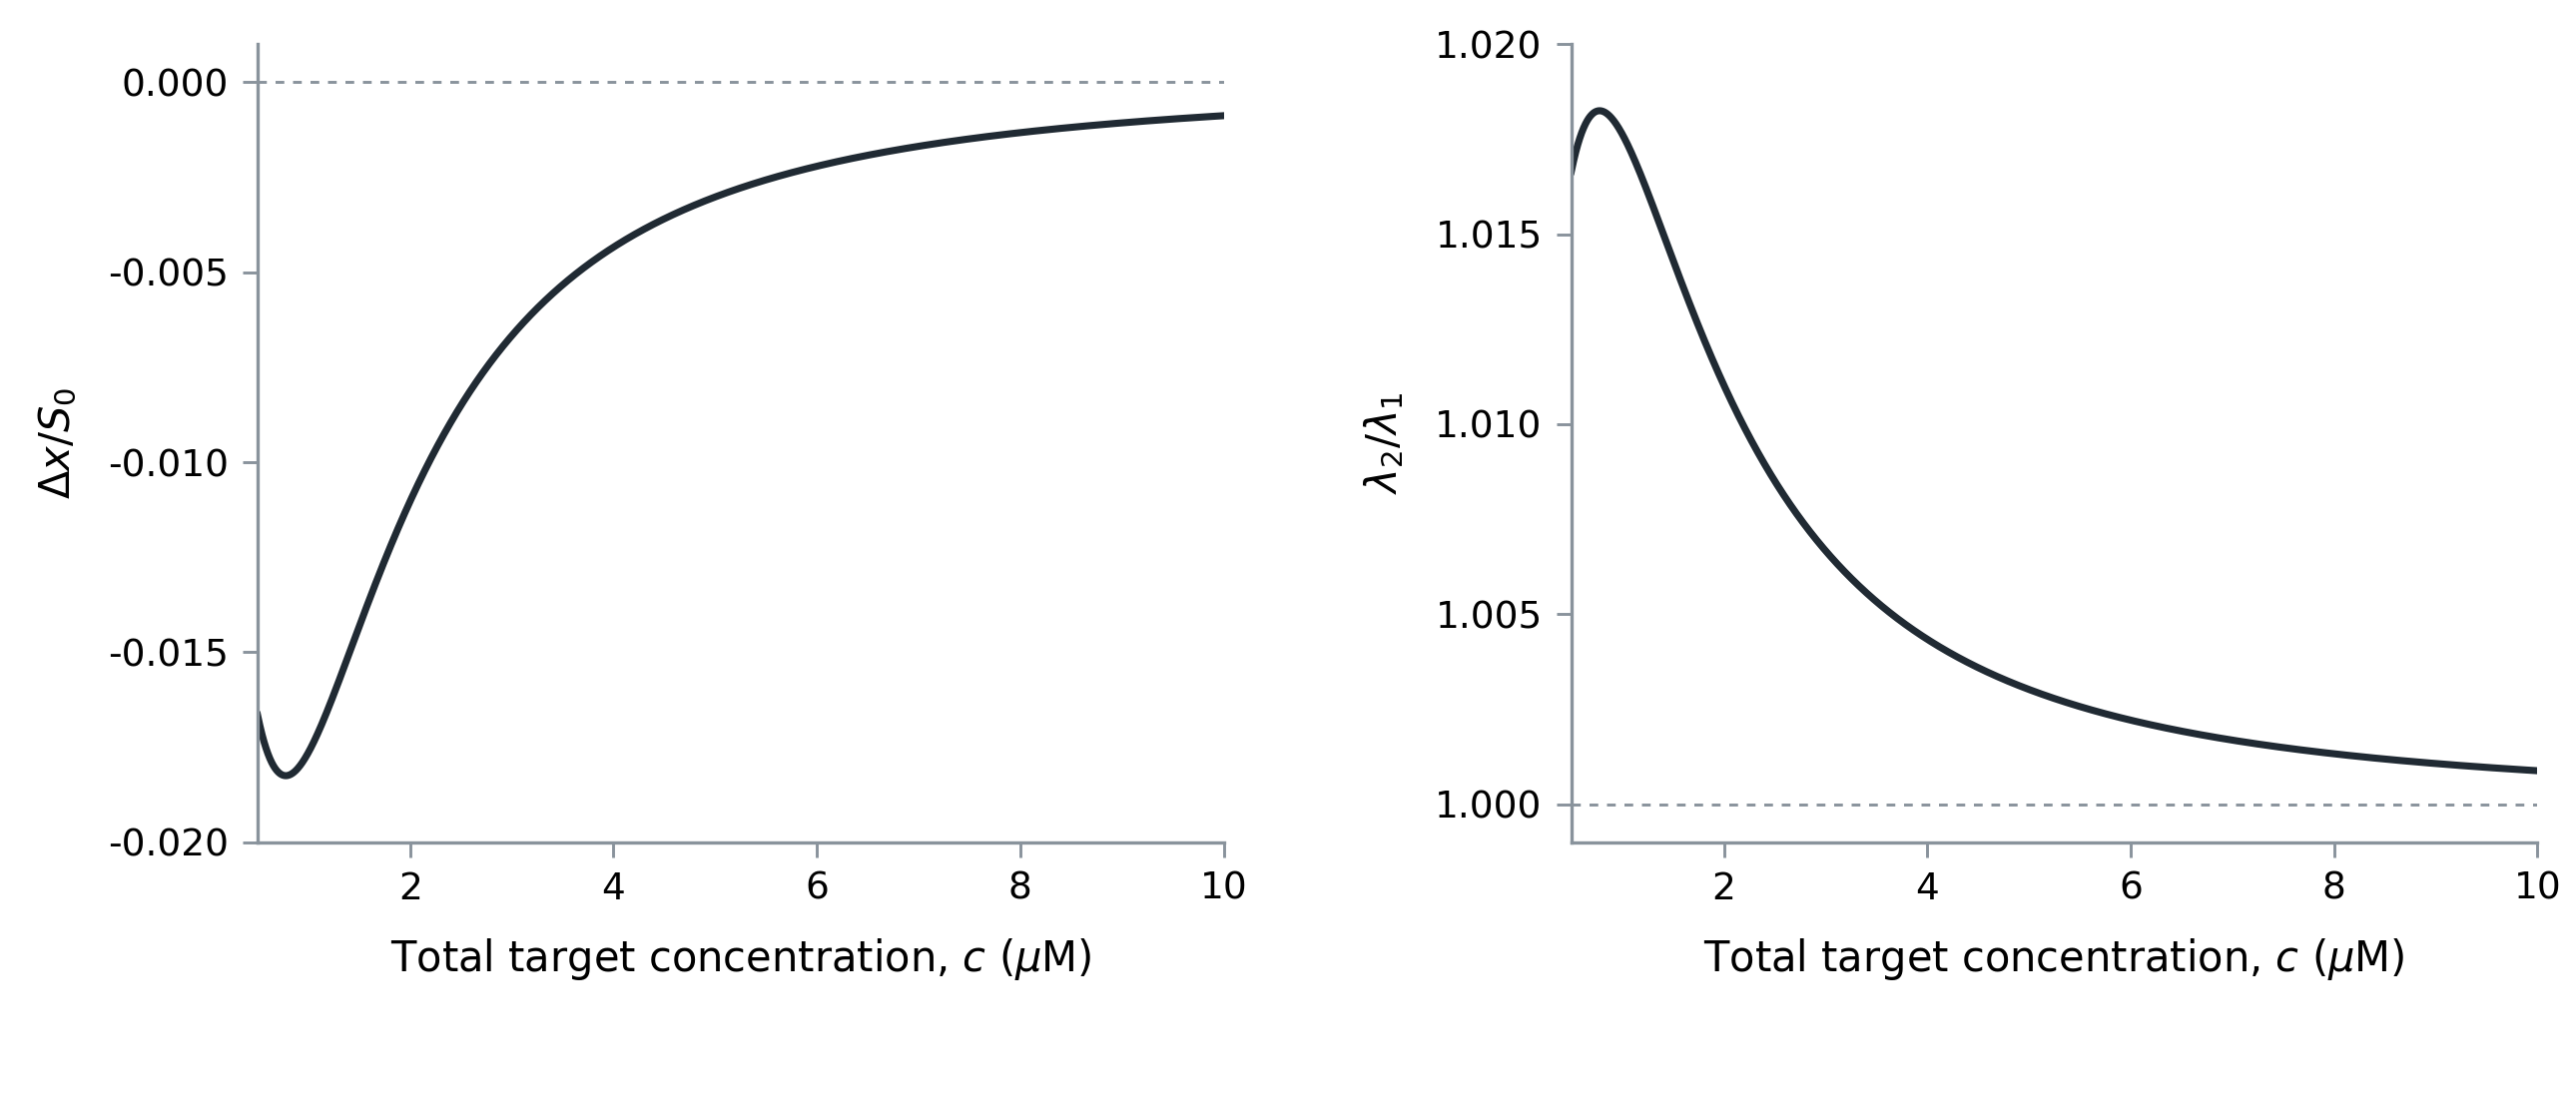
\includegraphics[width=0.9\linewidth]{Images/Comparison.png}
    \caption{Using the above established method, the ratio between the exact relaxation rate $\lambda_2$ and the linearized rate $\lambda_1$ is shown}
    \label{fig:ratio}
\end{figure}
\end{document}